%
% LaTeX-pohja opinnäytteille (kandit, gradut)
%
% Tekijät (ja jelppiä): Tero Vedenjuoksu, Markus Harju (Matemaattiset tieteet, Oulun Yliopisto)
\documentclass[12pt,a4paper,finnish,oneside,titlepage]{article}
\usepackage{tikz}
\usetikzlibrary{calc}
\usetikzlibrary{babel}
% Suomenkielinen tavutus ja ääkköset, valitse yksi näistä
%\usepackage[latin1]{inputenc}      % Linux
%\usepackage[ansinew]{inputenc}  % Windows, ansi
\usepackage[utf8]{inputenc}            % utf8, Windows ja Max OS X
% \usepackage[cp850]{inputenc}    % DOS

\usepackage{mathtools}
\usepackage{hyperref}
\usepackage{amsmath,algorithm,float,tabularx,amsfonts}
\usepackage{algpseudocode}
\makeatletter
\renewcommand{\ALG@name}{Algoritmi}
\newcommand{\multiline}[1]{%
    \begin{tabularx}{\dimexpr\linewidth-\ALG@thistlm}[t]{@{}X@{}}
        #1
    \end{tabularx}
}
\newcommand{\Input}[1]{\algrenewcommand{\alglinenumber}[1]{\textbf{Syöte:} \ \setcounter{ALG@line}{\numexpr##1-1}} #1}
\newcommand{\Step}[1]{\algrenewcommand{\alglinenumber}[1]{Askel ##1: } #1}
\newcommand{\NoNumber}{\algrenewcommand{\alglinenumber}[1]{\setcounter{ALG@line}{\numexpr##1-1} \ \ \ \ \ \ \ \ \ \ }}
\newcommand{\Output}[1]{\algrenewcommand{\alglinenumber}[1]{\textbf{Ulostulo:}\setcounter{ALG@line}{\numexpr##1-1}} #1}

\usepackage[T1]{fontenc}         
\usepackage[finnish]{babel}
% Paketti babel muuttaa myös kirjoitelmassa olevat nimikkeet kuten 'table of contents'
% vastaaviksi suomenkielisiksi nimikkeiksi

% PAKETIT
\usepackage{pgfplots}
\pgfplotsset{compat=1.6}
\pgfplotsset{soldot/.style={color=blue,only marks,mark=*}} \pgfplotsset{holdot/.style={color=blue,fill=white,only marks,mark=*}}
\usepackage{amsmath}             % AMS-LaTeX, matemaattisia makroja
\usepackage{amssymb}             % American mathematical Societyn tekemiä symboleita
\usepackage{amsfonts}            % American Mathematical Societyn fonttikokoelma 
                                 % matematiikkaa varten: liitutaulufontit yms.
\usepackage{latexsym}            % matemaattisia symboleita
\usepackage{amsthm}              % Paketti teoreemaympäristöille
%\usepackage{mathtools}           % Lisää työkaluja matemaattisten kaavojen kirjoittamiseen
                                 % vain yhtälött, joihin viitataan, numeroidaan
\usepackage{graphicx}            % paketti grafiikan lisäämiseen
\usepackage{import}

\usepackage{float}
\usepackage{amsmath} % for aligned
%\usepackage{amssymb} % for \mathbb
\usepackage{tikz}
%\usepackage{etoolbox} % for \ifthen
\usepackage{listofitems} % for \readlist to create arrays
\usetikzlibrary{arrows.meta} % for arrow size
\usepackage[outline]{contour} % glow around text
\contourlength{1.4pt}

\DeclareMathOperator*{\argmin}{argmin} % thin space, limits underneath in displays

\tikzset{>=latex} % for LaTeX arrow head
\usepackage{xcolor}
\colorlet{myred}{red!80!black}
\colorlet{myblue}{blue!80!black}
\colorlet{mygreen}{green!60!black}
\colorlet{myorange}{orange!70!red!60!black}
\colorlet{mydarkred}{red!30!black}
\colorlet{mydarkblue}{blue!40!black}
\colorlet{mydarkgreen}{green!30!black}
\tikzstyle{node}=[thick,circle,draw=myblue,minimum size=22,inner sep=0.5,outer sep=0.6]
\tikzstyle{node in}=[node,green!20!black,draw=mygreen!30!black,fill=mygreen!25]
\tikzstyle{node hidden}=[node,blue!20!black,draw=myblue!30!black,fill=myblue!20]
\tikzstyle{node convol}=[node,orange!20!black,draw=myorange!30!black,fill=myorange!20]
\tikzstyle{node out}=[node,red!20!black,draw=myred!30!black,fill=myred!20]
\tikzstyle{connect}=[thick,mydarkblue] %,line cap=round
\tikzstyle{connect arrow}=[-{Latex[length=4,width=3.5]},thick,mydarkblue,shorten <=0.5,shorten >=1]
\tikzset{ % node styles, numbered for easy mapping with \nstyle
  node 1/.style={node in},
  node 2/.style={node hidden},
  node 3/.style={node out},
}
\def\nstyle{int(\lay<\Nnodlen?min(2,\lay):3)} % map layer number onto 1, 2, or 3

%TEKSTIN ULKOASUUN VAIKUTTAVIA PARAMETREJA
%\linespread{1.3}                  % Riviväli. 1.3='riviväli 1.5' 1.6='riviväli 2'
\frenchspacing                    % normaali väli pisteen jälkeen; englanninkielisessä dokumentissa
\usepackage{tikz}
%OMIA MAKROJA

% Makroja lukujoukoille
\newcommand{\field}[1]{\mathbb{#1}}    % Makro lukujoukkojen määrittelyä varten
\newcommand{\N}{\field{N}}             % Luonnollisten lukujen joukko 
\newcommand{\Z}{\field{Z}}             % Kokonaislukujen joukko
\newcommand{\Q}{\field{Q}}             % Rationaalilukujen joukko
\newcommand{\R}{\field{R}}             % Reaalilukujen joukko
\newcommand{\C}{\field{C}}             % Kompleksilukujen joukko


% OMIA MATEMAATTISIA OPERAATTOREITA
\DeclareMathOperator{\re}{\mathrm{Re}} % Makro reaaliosaa varten
\DeclareMathOperator{\im}{\mathrm{Im}} % Makro imaginääriosaa varten
\DeclareMathOperator{\syt}{\mathrm{syt}} % Makro reaaliosaa varten
\DeclarePairedDelimiter\norm{\lVert}{\rVert}%

% TEOREEMAYMPÃRISTÖJÄ
\theoremstyle{plain}
\newtheorem{lause}{Lause}[section]     % Ympäristö lauseille, numerointi 2 numeroinen 
\newtheorem{lemma}[lause]{Lemma}       % Ympäristö lemmoille
\newtheorem{seur}[lause]{Seuraus}      % Ympäristö seurauksille, 

\theoremstyle{definition}
\newtheorem{maar}[lause]{Määritelmä}   % Ympäristö määritelmille
\newtheorem{esim}[lause]{Esimerkki}    % Ympäristö esimerkeille

\theoremstyle{remark}
\newtheorem{huom}[lause]{Huomautus}    % Ympäristö huomautuksille

%\numberwithin{equation}{section}       % yhtälöiden numerointi 2-numeroiseksi

% TAVUTUSVIHJEITÄ
%\hyphenation{jul-ki-suu-des-sa to-den-nä-köi-nen}

% huomaa, että hyphenation-ympäristö ei ymmärrä sanoja, 
% joissa on tavuviiva (esim. yli-ihminen). Tällöinin LaTeXia on käskettävä 
% leipätekstin seassa, käsky \- ilmoittaa mahdollisen 
% tavutuspaikan: y\-li-\-ih\-mi\-nen. Vaihtoehtoisesti voi käyttää käskyä
% "- joka tuottaa väliviivan, joka sallii tavutuksen muualla sanassa

\usetikzlibrary{calc}
\begin{document}
\begin{titlepage}
\vspace*{5.5cm}	  % tyhjää 5.5 cm , ilman tähteä käsky ei toimi sivun alussa
\begin{center}
\LARGE{\textbf{Myötäsyötteiset neuroverkot}}
\end{center}
\vfill    % tyhjää tilaa otsikon alle niin paljon kuin mahtuu
\begin{flushright}
LuK-tutkielma\\
Jimi Käyrä\\
Matemaattisten tieteiden yksikkö\\
Oulun yliopisto\\
Syksy 2022
\end{flushright}
\end{titlepage}

\tableofcontents
\newpage


\section*{Johdanto}
\addcontentsline{toc}{section}{Johdanto}
Tämän kandidaatintutkielman tavoitteena on perehtyä neuraalilaskentaan, joka on koneoppimisen alalla laajasti hyödynnetty ja erityisesti viime aikoina suosiotaan kasvattanut monipuolinen menetelmä. Neuraalilaskentaa toteutetaan neuroverkoilla, joista tässä tutkielmassa rajoitutaan tarkastelemaan niiden alalajia, myötäsyötteisiä neuroverkkoja. Yksinkertaisesta perusrakenteestaan huolimatta myötäsyötteisillä neuroverkoilla voidaan ratkaista varsin monimutkaisia koneoppimisen ongelmia.

Tutkielman ensimmäisessä luvussa esitetään lyhyt johdatus koneoppimiseen ja koneoppimisen ongelmien jaotteluun. Seuraavaksi toisessa luvussa siirrytään tarkastelemaan keinotekoisen neuronin rakennetta ja toimintaa, minkä jälkeen edetään kokonaisen, useista neuroneista koostuvan neuroverkon rakenteen ja toiminnan tarkasteluun. Viimeisessä luvussa tarkastellaan neuroverkon opettamista.

Tutkielman runkona on käytetty päälähdettä \cite{Z2b}, minkä lisäksi joissakin määritelmissä ja tulosten johtamisissa on käytetty lähteitä \cite{deriv}, \cite{net}, \cite{stanf}. Joitakin esimerkkejä ja merkintöjä on muokattu tutkielmaan paremmin sopiviksi, minkä lisäksi esimerkki 2.6 on laadittu kokonaan itse.

Olisi suotavaa, että tutkielman lukijalla olisi perustiedot lineaarialgebrasta, graafiteoriasta sekä differentiaalilaskennasta erityisesti derivoinnin ketjusäännön osalta. Lisäksi koneoppimisen perustuntemuksesta on apua aiheen taustan ja kontekstin hahmottamisessa.
\clearpage
\section{Koneoppiminen}\label{sec:ensimmainen}
Koneoppiminen voidaan käsittää tekoälyn osa-alueeksi, joka painottuu oppimiseen datan pohjalta. Eräs yleisesti käytetty määritelmä on seuraava:
\begin{center}
``A computer program is said to learn from \emph{experience} \(E\) with respect to some class of \emph{tasks} \(T\) and \emph{performance measure} \(P\), if its performance at tasks in \(T\), as measured by \(P\), improves with experience \(E\).`` \\ (Mitchell, 1997)
\end{center}
Koneoppimisessa on siis olennaisesti kyse algoritmeista, jotka kykenevät automaattisesti parantamaan suoriutumistaan (mitattuna mitalla \(P\)) tehtävissä \(T\) kokemuksen \(E\) avulla. Esimerkkinä voidaan tarkastella roskapostisuodatinta, jonka tehtävänä \(T\) on luokitella saapuvat sähköpostiviestit sen mukaan, ovatko ne roskapostia vai ei. Lisäksi mitaksi \(P\) valitaan oikein luokiteltujen viestien suhteellinen osuus kaikista viesteistä. Tällainen koneoppimisalgoritmi oppii kokemuksesta \(E\) ja parantaa suoriutumistaan nyt siten, että sähköpostin käyttäjä tarkistaa tehdyt luokittelut ja tarvittaessa korjaa niitä.

\subsection{Ohjattu ja ohjaamaton oppiminen}
Koneoppimisen ongelmat voidaan jaotella ohjatun ja ohjaamattoman oppimisen ongelmiin sen mukaan, minkälaista dataa algoritmilla on käytettävissä ja minkälainen ongelma on ratkaistavana.

Ohjatussa oppimisessa koneoppimismallia opetetaan opetusdatajoukolla \[L=\left\{(x^{(1)}, y^{(1)}), \ldots, (x^{(M)}, y^{(M)})\right\}\subset X\times Y,\] jossa \(x^{(i)}\in X\) on opetusesimerkin \(i\) piirrevektori ja \(y^{(i)}\in Y\) vastaava kohdemuuttujan arvo. Tavoitteena on etsiä sellainen funktio \(g : X\to Y\), että \(g(x)\) ennustaa mahdollisimman hyvin kohdemuuttujan todellisen, tuntemattoman arvon, kun \(x\in X\) on opetusdataan kuulumaton piirrevektori. Mallin opettamisen tavoitteena on siis säätää mallin parametrit siten, että tämä approksimointi olisi mahdollisimman tarkkaa.  Lisäksi ohjatun oppimisen ongelmat voidaan jakaa edelleen regressio- ja luokitteluongelmiin sen mukaan, ennustetaanko jatkuvaa vai diskreettiä muuttujaa. Ohjatun oppimisen mallia on havainnollistettu kuvassa 1.
\begin{center}
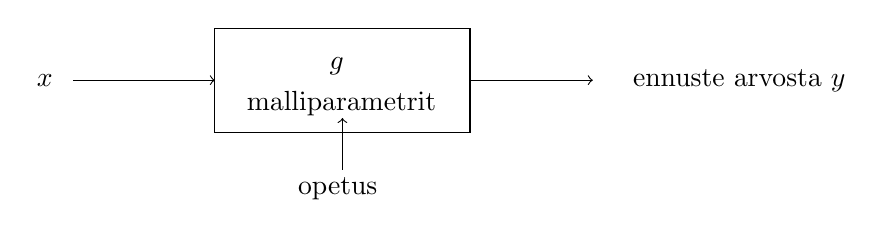
\begin{tikzpicture}[scale=1.2]
\node[] at (-1.8,0.75) {\(x\)};
\node[] at (5.55,0.74) {ennuste arvosta \(y\)};

\draw [-to](-1.5,0.75)--(0,0.75);
\draw [-to](2.7,0.75)--(4,0.75);

\filldraw[fill=none] (0,0.2) rectangle (2.7,1.3);
\draw [-to](1.35,-0.2)--(1.35,0.35);
\node[] at (1.3,-0.4) {opetus};

%\draw [-to](8.05,1.25)--(9.5,1.25);
\node[] at (1.29,0.9) {\(g\)};
\node[] at (1.34,0.5) {malliparametrit};
\end{tikzpicture}
\vspace{0.1in}
\\Kuva 1: Ohjatun oppimisen malli
\end{center}

Sen sijaan ohjaamattoman oppimisen ongelmissa kohdemuuttujan arvoja ei ole käytettävissä, vaan ainoastaan piirrevektorit \(x^{(1)}, \ldots, x^{(M)}\). Tällöin tavoitteena on, että koneoppimisalgoritmi kykenee jakamaan datan luokkiin itsenäisesti, jolloin saadaan tietoa datajoukon rakenteesta. Ohjaamattoman oppimisen käyttökohteisiin lukeutuvatkin erityisesti klusterointiongelmat, joissa data pyritään jakamaan tyypillisesti ennalta määrittelemättömiin ryppäisiin siten, että yksittäisen ryppään datapisteet ovat keskenään samankaltaisia, mutta eri ryppäät eroavat toisistaan mahdollisimman paljon. Toinen tärkeä ohjaamattoman oppimisen käyttökohde on dimensionaalisuuden vähentäminen, jonka tavoitteena on esittää korkeadimensioinen data pienemmässä määrässä ulottuvuuksia.

\subsection{Ali- ja ylioppiminen}
Alioppimisella (\emph{underfitting}) tarkoitetaan ilmiötä, jossa malli ei kykene oppimaan datan rakennetta riittävän hyvin. Tällöin mallin tekemä ennustevirhe jää suureksi sekä opetus- että testausdatalle. Alioppimiseen voi johtaa esimerkiksi liian yksinkertaisen mallin valinta tai opetusdatajoukon liian pieni koko.

Toisaalta opettaminen voi johtaa myös siihen, että malli suoriutuu erittäin hyvin opetusdatalla, mutta ennustaminen epäonnistuu testausdatalle eli mallin yleistämiskyky (\emph{generalizability}) jää heikoksi. Tällöin puhutaan ylioppimisesta (\emph{overfitting}). Ylioppimista voi aiheuttaa mm. huonolaatuinen opetusdata, jolloin malli oppii mukailemaan liikaa datassa esiintyvää kohinaa.
\begin{center}
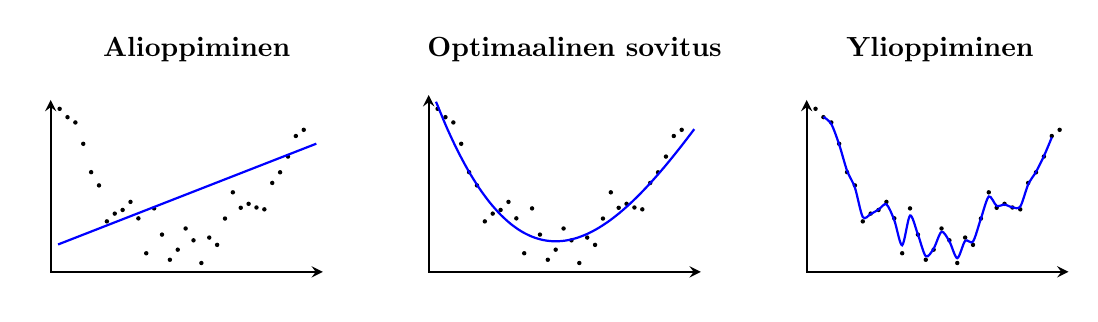
\begin{tikzpicture}[scale=0.8,declare function={f(\x)=0.5*pow(abs(\x-2),2)-0.06*pow(\x-2,3);}]
 \pgfmathsetseed{3333}
 \foreach \Z in {1,...,32}
 {\pgfmathsetmacro{\X}{\Z/8}
 \pgfmathsetmacro{\Y}{f(\X)+0.9*rnd}
 \ifnum\Z=1
  \xdef\LstOne{(\X,\Y)}
  \xdef\LstTwo{"(\X,\Y)"}
 \else
  \xdef\LstOne{\LstOne (\X,\Y)}
  \xdef\LstTwo{\LstTwo,"(\X,\Y)"}
 \fi}
 \begin{scope}[local bounding box=over,xshift=-5cm]
 \foreach \Z in {1,...,30}
 {\pgfmathsetmacro{\Last}{{\LstTwo}[\Z-1]}
 \pgfmathsetmacro{\Current}{{\LstTwo}[\Z]}
 \pgfmathsetmacro{\Next}{{\LstTwo}[\Z+1]}
  \edef\temp{\noexpand\path ($0.8*\Current+0.1*\Last+0.1*\Next$)   coordinate 
  (p\Z);}
  \temp
  \ifnum\Z=1
  \xdef\LstThree{(p\Z)}
  \else
  \xdef\LstThree{\LstThree (p\Z)}
  \fi
  }
 \foreach \Z in {1,...,32}
 {\pgfmathsetmacro{\Coor}{{\LstTwo}[\Z-1]}
 \fill \Coor circle[radius=1pt];
 }
 \draw[thick,blue] plot[smooth] coordinates \LstThree;
 \end{scope}
 %
 \begin{scope}[local bounding box=good,xshift=-11cm]
 \foreach \Z in {1,...,32}
 {\pgfmathsetmacro{\Coor}{{\LstTwo}[\Z-1]}
 \fill \Coor circle[radius=1pt];
 }
 \draw[thick,blue] plot[smooth,domain=0.1:4.2,variable=\x] (\x,{f(\x)+0.45});
 \end{scope}
 %
 \begin{scope}[local bounding box=under,xshift=-17cm]
 \foreach \Z in {1,...,32}
 {\pgfmathsetmacro{\Coor}{{\LstTwo}[\Z-1]}
 \fill \Coor circle[radius=1pt];
 }
 \draw[thick,blue] (0.1,0.4) -- (4.2,2);
 \end{scope}
 %
 \foreach \X in {over,good,under}
 {
 ([xshift=3pt,yshift=-3pt]\X.south east);
 \draw[stealth-stealth,thick] ([xshift=-3pt,yshift=3pt]\X.north west) node[left=5pt, below=40pt]{} 
 |- ([xshift=3pt,yshift=-3pt]\X.south east) node[left=65pt, below=1pt]{};}

 \node[] at (-14.7,3.5) {\normalsize \textbf{Alioppiminen}};
  \node[] at (-8.7,3.5) {\normalsize \textbf{Optimaalinen sovitus}};
\node[] at (-2.9,3.5) {\normalsize \textbf{Ylioppiminen}};
\end{tikzpicture}
\vspace{0.1in}
\\Kuva 2: Ali- ja ylioppiminen
\end{center}

\section{Neuroverkon rakenne ja toiminta}\label{sec:toinen}
Tässä luvussa tarkastellaan keinotekoista neuroverkkoa, joka käsitetään nyt ohjatun oppimisen malliksi. Keinotekoiset neuroverkot ovat monipuolisia koneoppimisen malleja, jotka pohjautuvat löyhästi biologisen hermoston toimintaan. Hermoston tavoin myös keinotekoinen neuroverkko koostuu neuroneista, jotka ovat toisiinsa kytkettyjä ja välittävät toisilleen tietoa. Lisäksi oppimisen taustalla on jokseenkin vastaava pääperiaate: kuten hermostossa, myös keinotekoisessa neuroverkossa oppiminen perustuu siihen, että tietyt neuronien väliset yhteydet vahvistuvat. Keinotekoisten neuroverkkojen etuihin lukeutuvatkin erityisesti suuri mukautuvuus ja monikäyttöisyys.

\subsection{Keinotekoinen neuroni}
Tarkastellaan ensin keinotekoista neuronia, joka on neuroverkkojen perusyksikkö. Monimutkaisemmat neuroverkot koostuvat useista neuroneista, jotka muodostavat erilaisia kokonaisuuksia verkon arkkitehtuurista riippuen.

Kuvassa 3 esitetty yksittäinen neuroni saa syötteekseen vektorin \(x=(x_1, x_2, \ldots, x_n)^{\top}\in \R^n\) ja painottaa jokaista komponenttia painokertoimella \(w_i\), \(i=1, 2, \ldots, n\). Painotetut kertoimet summataan ja saatuun summaan lisätään bias-termi \(b\). Lopuksi tulos syötetään aktivaatiofunktiolle \(f : \R\to \R\). Näin ollen neuronin lähdöksi saadaan \[h_{w,b}(x)=f\left(b+\sum_{i=1}^{n} w_i x_i\right)=f\left(w^{\top}x+b\right),\]
missä summaus on esitetty painovektorin \(w=(w_1, w_2, \ldots, w_n)^{\top}\in \R^n\) ja syötevektorin \(x\) sisätulona. Neuroni siis saa syötteekseen \(n\)-pituisen vektorin ja tuottaa siitä skalaariluvun.

\begin{center}
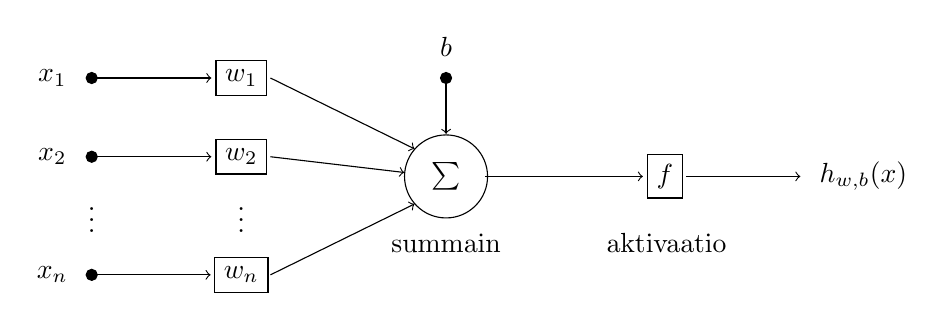
\begin{tikzpicture}
\node[] at (0,0) {\(x_n\)};
\draw [-to](0.5,0)--(2.01,0);
\filldraw (0.5,0) circle (2pt);
\node[draw] at (2.4,0) {\(w_n\)};

\node[] at (0,1.5) {\(x_2\)};
\draw [-to](0.5,1.5)--(2.02,1.5);
\filldraw (0.5,1.5) circle (2pt);
\node[draw] at (2.4,1.5) {\(w_2\)};

\node[] at (0,2.5) {\(x_1\)};
\draw [-to](0.5,2.5)--(2.02,2.5);
\filldraw (0.5,2.5) circle (2pt);
\node[draw] at (2.4,2.5) {\(w_1\)};

\node[] at (2.4,0.8) {\(\vdots\)};
\node[] at (0.5,0.8) {\(\vdots\)};

\draw (5,1.25) circle (15pt);
\draw [-to](5.5,1.25)--(7.5,1.25);
\node[draw] at (7.78,1.25) {\(f\)};
\node[] at (7.8,0.4) {aktivaatio};

\draw [-to](5,2.5)--(5,1.79);
\filldraw (5,2.5) circle (2pt);
\node[] at (5,2.9) {\(b\)};

\draw [-to](2.77,2.5)--(4.6,1.6);
\draw [-to](2.77,1.5)--(4.47,1.3);
\draw [-to](2.77,0)--(4.6,0.9);

\node[] at (5,1.25) {\(\sum\)};
\node[] at (5,0.4) {summain};

\draw [-to](8.05,1.25)--(9.5,1.25);
\node[] at (10.3,1.25) {\(h_{w,b}(x)\)};
\end{tikzpicture}
\vspace{0.1in}
\\Kuva 3: Keinotekoisen neuronin rakenne
\end{center}

\subsubsection{Aktivaatiofunktio}
Havaitaan, että summaimen lähtö \(w^{\top}x+b\) on syötevektorin \(x\) affiini muunnos. Jotta neuronilla olisi kuitenkin mahdollista mallintaa myös epälineaarisia riippuvuuksia, tarvitaan aktivaatiofunktiota \(f\).

Aktivaatiofunktio \(f\) valitaan usein siten, että se mallintaa biologisen neuronin toimintaa: kun aktivaatiofunktion saama syöte saavuttaa kynnysarvon, neuroni aktivoituu. Yksinkertaisimmillaan tällainen kynnystys voidaan toteuttaa binäärisellä yksikköaskelfunktiolla \[f_{\text{b}}(z)=\begin{cases} 1, &\text{kun }z\geq 0\\ 0 &\text{muulloin.}\end{cases}\]

Usein on kuitenkin tarpeen, että aktivaatiofunktio on diskreetin sijaan jatkuva. Binääriseen askelfunktioon verrattuna sigmoidifunktion \[f_{\text{s}}(z)=\frac{1}{1+\text{e}^{-z}}\]
etuina on mm. jatkuva vaste askelmaisen sijaan ja derivoituvuus jokaisessa kohdassa. Sigmoidifunktio soveltuu erityisesti todennäköisyyksien ennustamiseen, sillä \(0<f_\text{s}(z)<1\) kaikilla \(z\in \R\) ja jatkuvana funktiona se saavuttaa kaikki arvot väliltä \(]0, 1[\).

Etenkin monimutkaisemmissa, useista kerroksista koostuvissa neuroverkoissa käytetään usein ReLU-aktivaatiofunktiota (rectified linear unit)
\[f_{\text{R}}(z)=\text{max}(0, z)=\begin{cases} z, &\text{kun } z\geq 0\\ 0 &\text{muulloin.} \end{cases}\]
Sigmoidifunktioiden tavoin ReLU on jatkuva, mutta se saavuttaa kaikki arvot väliltä \([0, \infty[\) ja on siten rajoittamaton. Rajoittamattomuudesta voi olla etua erityisesti verkon opettamisessa.

Aktivaatiofunktioiden kuvaajat on esitetty kuvassa 2.

\begin{center}
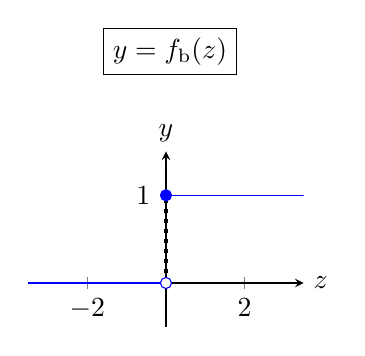
\begin{tikzpicture}[scale=1]
\node[draw] at (1.8,3.5) {\(y=f_\text{b}(z)\)};
\begin{axis}[height=1.5in,width=2in,axis x line=center,
  axis y line=center,
  xtick={-3,-4,...,3},
  ytick={0,1},
  xlabel={$z$},
  ylabel={$y$},
  xlabel style={right},
  ylabel style={above},
  xmin=-3.5,
  xmax=3.5,
  ymin=-0.5,
  ymax=1.5]
\addplot[domain=-5:0,blue] {0};
\addplot[domain=0:5,blue] {1};
%\addplot[domain=4:6,blue] {x};
%\addplot[domain=6:10,blue] {-5};
\draw[dotted,ultra thick] (axis cs:0,0) -- (axis cs:0,1);
\addplot[holdot] coordinates{(0,0)};
\addplot[soldot] coordinates{(0,1)};
\end{axis}
\end{tikzpicture}
\quad
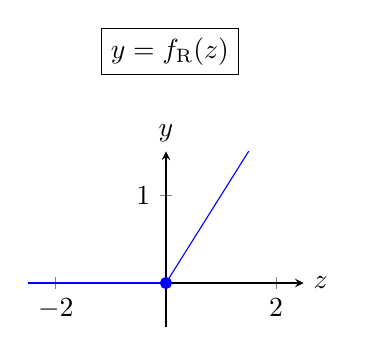
\begin{tikzpicture}[scale=1]
\node[draw] at (1.8,3.5) {\(y=f_\text{R}(z)\)};
\begin{axis}[height=1.5in,width=2in,axis x line=center,
  axis y line=center,
  xtick={-2,2},
  ytick={0,1},
  xlabel={$z$},
  ylabel={$y$},
  xlabel style={right},
  ylabel style={above},
  xmin=-2.5,
  xmax=2.5,
  ymin=-0.5,
  ymax=1.5]
\addplot[domain=-5:0,blue] {0};
\addplot[domain=0:5,blue] {x};
%\addplot[domain=4:6,blue] {x};
%\addplot[domain=6:10,blue] {-5};
\addplot[soldot] coordinates{(0,0)};
\end{axis}
\end{tikzpicture}
\quad
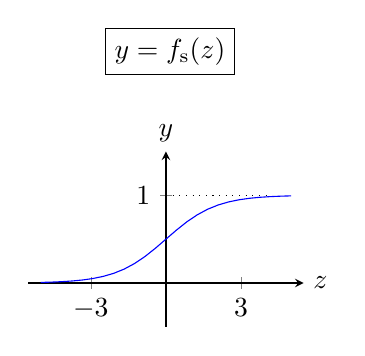
\begin{tikzpicture}[scale=1]
\node[draw] at (1.8,3.5) {\(y=f_\text{s}(z)\)};
\begin{axis}[height=1.5in,width=2in,axis x line=center,
  axis y line=center,
  xtick={-3,3},
  ytick={0,1},
  xlabel={$z$},
  ylabel={$y$},
  xlabel style={right},
  ylabel style={above},
  xmin=-5.5,
  xmax=5.5,
  ymin=-0.5,
  ymax=1.5]
  
\addplot[domain=-5:5,blue] {1 / (1 + exp(-x))};
%\addplot[domain=4:6,blue] {x};
%\addplot[domain=6:10,blue] {-5};
\draw[dotted] (axis cs:0,1) -- (axis cs:4,1);
\end{axis}
\end{tikzpicture}
\vspace{0.1in}
\\Kuva 4: Erilaisia aktivaatiofunktioita
\end{center}

\subsubsection{Bias}
Bias-termin \(b\) avulla voidaan säätää neuronin aktivoitumiseen vaadittavaa kynnystä. Tarkastellaan esimerkkinä neuronia, jonka aktivaatiofunktiona on käytetty binääristä askelfunktiota \(f_\text{b}\). Tällöin neuronin lähtö muuttuu arvosta 0 arvooon 1, kun summaimen lähtö \(w^{\top} x\) saavuttaa arvon 0, ts. \[f_\text{b}\left(w^{\top} x\right)=\begin{cases} 1, &\text{kun }w^{\top} x\geq 0 \\ 0 &\text{muulloin.}\end{cases}\]

Usein on kuitenkin tarpeen säätää aktivaatiokynnystä neuronikohtaisesti (aktivaatiofunktion pysyessä samana). Tämä on mahdollista toteuttaa bias-termin avulla: kun summaimen lähtöön lisätään \(b\), saadaan \[f_\text{b}\left(w^{\top} x+b\right)=\begin{cases} 1, &\text{kun }w^{\top} x+b\geq 0 \\ 0 &\text{muulloin}\end{cases}=\begin{cases} 1, &\text{kun }w^{\top} x\geq -b \\ 0 &\text{muulloin.}\end{cases}\]
Valitaan nyt \(b\) siten, että \(b<0\). Tällöin havaitaan, että neuroni aktivoituu vasta, kun summaimen lähtö saavuttaa kynnysarvon \(|b|\).

Käytännössä bias-termi siis mahdollistaa aktivaatiofunktion siirron vaakasuunnassa, kun taas painojen \(w_i\) varioinnilla voidaan muuttaa aktivaatiofunktion jyrkkyyttä. Tätä on havainnollistettu kuvassa 3 aktivaatiofunktiolle \(f_\text{s}\). Ensimmäisessä kuvaajassa on esitetty aktivaatiofunktion lähtö \(f_\text{s}(x_1)\), jossa syötteen painokerroin on 1 ja bias 0. Toisessa kuvaajassa painokertoimeksi on asetettu \(w_1=2\), mikä ilmenee kuvaajan skaalautumisena vaakasuunnassa eli jyrkkyyden muuttumisena. Viimeisessä kuvaajassa painokertoimen varioinnin lisäksi on asetettu bias \(b=-2\), minkä vaikutus näkyy kuvaajan siirtymisenä vaakasuunnassa.

\begin{center}
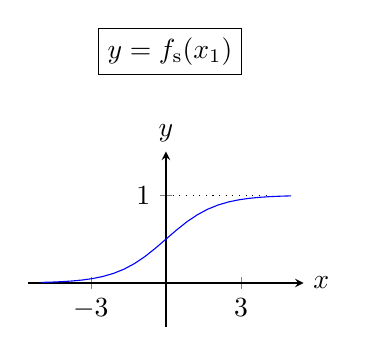
\begin{tikzpicture}[scale=1]
\node[draw] at (1.8,3.5) {\(y=f_\text{s}(x_1)\)};
\begin{axis}[height=1.5in,width=2in,axis x line=center,
  axis y line=center,
  xtick={-3,3},
  ytick={0,1},
  xlabel={$x$},
  ylabel={$y$},
  xlabel style={right},
  ylabel style={above},
  xmin=-5.5,
  xmax=5.5,
  ymin=-0.5,
  ymax=1.5]
  
\addplot[domain=-5:5,blue] {1 / (1 + exp(-x))};
%\addplot[domain=4:6,blue] {x};
%\addplot[domain=6:10,blue] {-5};
\draw[dotted] (axis cs:0,1) -- (axis cs:4,1);
\end{axis}
\end{tikzpicture}
\quad
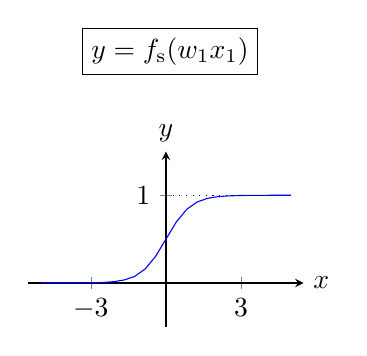
\begin{tikzpicture}[scale=1]
\node[draw] at (1.8,3.5) {\(y=f_\text{s}(w_1 x_1)\)};
\begin{axis}[height=1.5in,width=2in,axis x line=center,
  axis y line=center,
  xtick={-3,3},
  ytick={0,1},
  xlabel={$x$},
  ylabel={$y$},
  xlabel style={right},
  ylabel style={above},
  xmin=-5.5,
  xmax=5.5,
  ymin=-0.5,
  ymax=1.5]
  
\addplot[domain=-5:5,blue] {1 / (1 + exp(-(2*x)))};
%\addplot[domain=4:6,blue] {x};
%\addplot[domain=6:10,blue] {-5};
\draw[dotted] (axis cs:0,1) -- (axis cs:4,1);
\end{axis}
\end{tikzpicture}
\quad
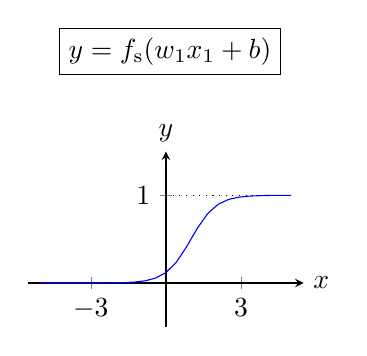
\begin{tikzpicture}[scale=1]
\node[draw] at (1.8,3.5) {\(y=f_\text{s}(w_1 x_1+b)\)};
\begin{axis}[height=1.5in,width=2in,axis x line=center,
  axis y line=center,
  xtick={-3,3},
  ytick={0,1},
  xlabel={$x$},
  ylabel={$y$},
  xlabel style={right},
  ylabel style={above},
  xmin=-5.5,
  xmax=5.5,
  ymin=-0.5,
  ymax=1.5]
  
\addplot[domain=-5:5,blue] {1 / (1 + exp(-(2*x-2)))};
%\addplot[domain=4:6,blue] {x};
%\addplot[domain=6:10,blue] {-5};
\draw[dotted] (axis cs:0,1) -- (axis cs:4,1);
\end{axis}
\end{tikzpicture}
\vspace{0.1in}
\\Kuva 5: Painon ja bias-termin vaikutus aktivaatiofunktioon
\end{center}

\subsection{Verkon rakenne}
Edellä tarkasteltiin keinotekoista neuronia, joka voidaan mieltää yhdestä neuronista koostuvaksi neuroverkoksi. Monimutkaisemmat neuroverkot koostuvat useista yksittäisistä neuroneista, jotka on kytketty toisiinsa eri tavoin ja välittävät toisilleen tietoa. Neuroverkkojen yhteydessä keinotekoisia neuroneja kutsutaan usein verkkoteorian termein solmuiksi (\textit{node}).

Neuroverkon rakenne voidaan kuvata tarkasti sen arkkitehtuurin avulla. Arkkitehtuuri määrittää mm. neuronien järjestyksen ja neuronien väliset yhteydet. Tämän pohjalta voidaan asettaa seuraava määritelmä.

\begin{maar}\label{maar:arc}
Neuroverkon arkkitehtuuri voidaan kuvata järjestettynä nelikkona \((I, L, O, E)\), jossa \(I\) on syötepaikkojen joukko, \(L\) laskentayksikkösolmujen joukko, \(O\) lähtöpaikkojen joukko ja \(E\) joukko, joka koostuu painotetuista, suunnatuista linkeistä. Linkki on kolmikko \((u, v, w)\), jossa \(u\in I\cup L\), \(v\in L\cup O\) ja \(w\in \R\). \cite{net}
\end{maar}

\begin{huom}
Syöte- ja lähtöpaikat on esitetty tässä erillisinä osina laskentayksikkösolmuista, sillä laskentayksikkösolmuista poiketen ne eivät suorita varsinaista laskentaa.
\end{huom}

Tarkastellaan nyt kerroksittaista arkkitehtuuria, jossa laskentayksikkösolmujen joukko \(L\) voidaan osittaa \(n_l\) osajoukoksi \(L_1, L_2, \ldots, L_{n_l}\) siten, että joukon \(L_2\) solmuihin on linkki ainoastaan joukon \(L_1\) solmuista ja yleisesti joukon \(L_{i+1}\) solmuihin on linkki ainoastaan joukon \(L_{i}\) solmuista. Kutsutaan myös joukkoa \(L_i\) kerrokseksi. Lisäksi syötesolmuista \(I\) on linkki ainoastaan joukon \(L_1\) solmuihin ja vastaavasti lähtösolmuihin \(O\) on linkki ainoastaan joukon \(L_{n_l}\) solmuista.

Tässä joukkoa \(L_1\) sanotaan syötekerrokseksi, sillä sen neuronit käyttävät syötteenään suoraan syötepaikoista \(I\) saatavaa verkon syötettä. Vastaavasti viimeistä joukkoa \(L_{n_l}\) sanotaan lähtökerrokseksi, sillä tämän kerroksen neuronien lähdöistä saadaan koko verkon lähtö, joka on luettavissa lähtöpaikoista \(O\). Väliin jääviä kerroksia \(L_2, \ldots, L_{n_l-1}\) kutsutaan piilokerroksiksi, sillä ne ovat kiinteämmin osa verkon sisäistä rakennetta eivätkä ne käsittele suoraan verkon syötettä tai tuota verkon lähtöä.

\begin{maar}\label{maar:grad}
Neuroverkko on myötäsyötteinen (\textit{feed-forward}) täsmälleen silloin, kun se ei sisällä syklejä.
\end{maar}

Havaitaan, että edellä kuvaillun kerrosmaisen arkkitehtuurin mukaiset neuroverkot ovat myötäsyötteisiä: linkkejä on ainoastaan kahden peräkkäisen kerroksen välillä, joten verkkoon ei muodostu syklejä.

Neuroverkossa kahden neuronin \(u\) ja \(v\) välisellä linkillä \((u, v, w)\) on painokerroin \(w\). Erityisesti havaitaan, että linkit ovat suunnattuja eli \((u, v, w)\) on eri linkki kuin \((v, u, w)\). Myötäsyötteisessä, kerrosmaisessa neuroverkossa linkki voi suuntautua ainoastaan seuraavan kerroksen neuroniin eli jos \(u\in L_i\), on oltava \(v\in L_{i+1}\), jotta linkki \((u, v, w)\) voisi olla olemassa.

Tarkastellaan tässä täysin kytkettyä myötäsyötteistä neuroverkkoa, jossa jokainen kerroksen \(i\) solmu on kytketty jokaiseen seuraavan kerroksen \(i+1\) solmuun. Olkoon nyt \(w_{ij}^{(l)}\) tämän kerroksen \(l+1\) solmua \(i\) ja kerroksen \(l\) solmua \(j\) yhdistävän linkin paino. Vastaavasti merkitään, että \(b_i^{(l)}\) on kerroksen \(l+1\) solmun \(i\) bias-termi. Kerroksen \(l\) neuronin \(j\) lähdölle käytetään merkintää \(h_j^{(l)}\). Merkitään lisäksi kerroksen \(l\) neuronien lukumäärää \(s_l=\left|L_l\right|\).

\begin{esim}
Kuvassa 6 on esitetty neuroverkko, joka koostuu syöte- ja lähtökerroksista \(1\) ja \(3\) sekä yhdestä piilokerroksesta \(2\). Syötekerros koostuu neljästä neuronista, jotka on numeroitu \(1, \ldots, 4\). Lisäksi havaitaan, että verkko on myötäsyötteinen: verkossa ei ole syklejä, vaan kunkin kerroksen neuroneilla on linkit ainoastaan seuraavan kerroksen neuroneihin.

Verkon syötepaikkoihin \(I\) on syötetty syötevektori \(x=(x_1, x_2, x_3, x_4)\), jonka komponentit toimivat syötekerroksen neuronien syötteinä. Vastaavasti verkon lähtöpaikoissa sijaitseva verkon lähtö saadaan lähtökerroksen neuronien lähtöinä \(h_1^{(3)}\) ja \(h_2^{(3)}\).
\begin{center}
\tikzset{%
  every neuron/.style={
    circle,
    draw,
    minimum size=1cm
  },
  neuron missing/.style={
    draw=none, 
    scale=3,
    text height=0.333cm,
    execute at begin node=\color{black}$\vdots$
  },
}

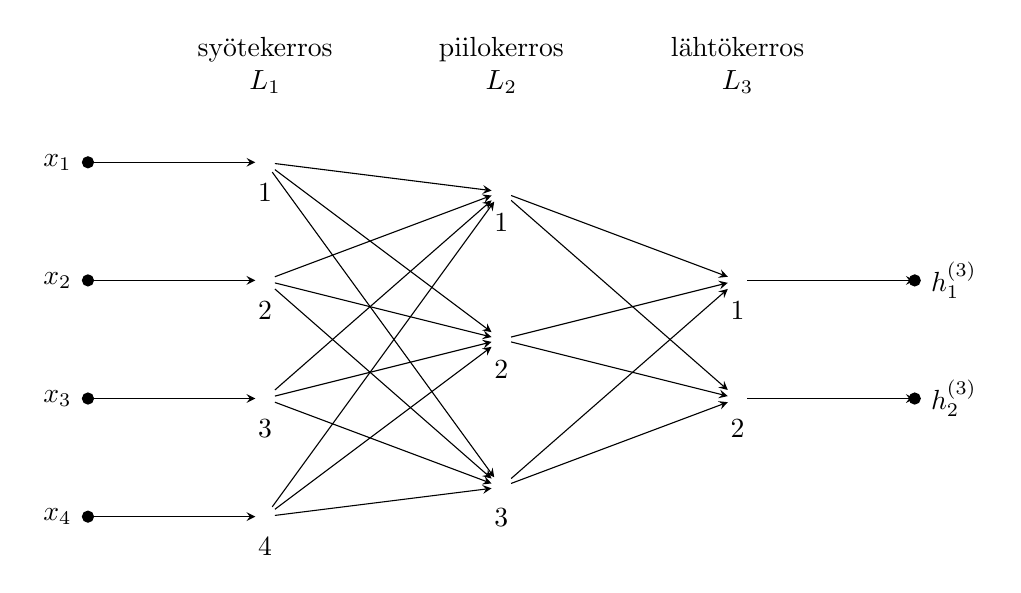
\begin{tikzpicture}[x=1.5cm, y=1.5cm, >=stealth]


\foreach \m/\l [count=\y] in {1,2,3,4}
  \node [every neuron/.try, neuron \m/.try] (input-\m) at (0,2.5-\y) {};

\foreach \m [count=\y] in {1,2,3}
  \node [every neuron/.try, neuron \m/.try ] (hidden-\m) at (2,2.5-\y*1.25) {};

\foreach \m [count=\y] in {1,2}
  \node [every neuron/.try, neuron \m/.try ] (output-\m) at (4,1.5-\y) {};

\foreach \l [count=\i] in {1,2,3,4}
  \draw [<-] (input-\i) -- ++(-1.5,0)
    node [left,inner sep=0.2cm] {$x_\l$};
  %\node[] at (0,1.5) {\(x_2\)};
  
\foreach \l [count=\i] in {1,2,3,4}
  \filldraw (input-\i)++(-1.5,0) circle (2pt);
    
\foreach \l [count=\i] in {1,2,3,4} % syötekerroksen numerot
  \node [shift={(0,-0.34)}] at (input-\i.north) {\l};

\foreach \l [count=\i] in {1,2,3} % piilokerroksen numerot
  \node [shift={(0,-0.34)}] at (hidden-\i.north) {\l};
  
\foreach \l [count=\i] in {1,2} % lähtökerroksen numerot
  \node [shift={(0,-0.34)}] at (output-\i.north) {\l};

\foreach \l [count=\i] in {1,2}
  \draw [->] (output-\i) -- ++(1.5,0)
    node [right,inner sep=0.2cm] {$h_\l^{(3)}$};


\foreach \l [count=\i] in {1,2}
    \filldraw (output-\i)++(1.5,0) circle (2pt);

\foreach \i in {1,...,4}
  \foreach \j in {1,...,3}
    \draw [->] (input-\i) -- (hidden-\j);

\foreach \i in {1,...,3}
  \foreach \j in {1,...,2}
    \draw [->] (hidden-\i) -- (output-\j);

\foreach \l [count=\x from 0] in {syötekerros\\ \(L_1\), piilokerros\\ \(L_2\), lähtökerros\\ \(L_3\)}
  \node [align=center, above] at (\x*2,2) {\l};

\end{tikzpicture}
\vspace{0.1in}
\\Kuva 6: Esimerkki neuroverkosta
\end{center}
\end{esim}

\subsection{Myötäsyöttöprosessi}
Myötäsyöttöprosessin (\textit{feed-forward pass}) avulla saadaan määritettyä vaiheittain verkon lähtö. Prosessissa lähdetään liikkeelle verkon syötteestä ja lasketaan kerroksittain jokaisen neuronin lähdöt, joita käytetään edelleen seuraavan kerroksen neuronien syötteinä. Näin jatkaen edetään lopulta lähtökerrokseen, josta voidaan lukea koko verkon lähtö.

Tarkastellaan esimerkkinä myötäsyöttöprosessia kuvan 6 neuroverkolle. Kukin syötekerroksen \(1\) neuroni \(i\) saa syötteekseen verkon syötteen \(x_i\) ja tuottaa tämän lähdökseen sellaisenaan, ts. \(h_i^{(1)}=x_i\) kaikille \(i=1, 2, 3, 4\). Kerroksen \(2\) neuroni \(1\) saa nyt syötteekseen edellisen kerroksen \(1\) neuronien lähdöt \(h_1^{(1)}\), \(h_2^{(1)}\), \(h_3^{(1)}\), \(h_4^{(1)}\) ja painottaa niitä vastaavilla painokertoimilla \(w_{11}^{(1)}\), \(w_{12}^{(1)}\), \(w_{13}^{(1)}\), \(w_{14}^{(1)}\). Painotettujen lähtöjen summaan lisätään bias \(b_1^{(1)}\) ja tulos syötetään aktivaatiofunktiolle \(f\). Tällä tavoin kerroksen \(2\) neuronien lähdöiksi saadaan siis 
\[\begin{align*}
    h_1^{(2)}&=f\left(w_{11}^{(1)} h_1^{(1)} + w_{12}^{(1)} h_2^{(1)} + w_{13}^{(1)} h_3^{(1)} + w_{14}^{(1)} h_4^{(1)} +b_1^{(1)}\right), \\
    h_2^{(2)}&=f\left(w_{21}^{(1)} h_1^{(1)} + w_{22}^{(1)} h_2^{(1)} + w_{23}^{(1)} h_3^{(1)}+w_{24}^{(1)} h_4^{(1)}+b_2^{(1)}\right), \\
    h_3^{(2)}&=f\left(w_{31}^{(1)} h_1^{(1)} + w_{32}^{(1)} h_2^{(1)} + w_{33}^{(1)} h_3^{(1)}+w_{34}^{(1)}h_4^{(1)}+b_3^{(1)}\right).
\end{align*}\]
Syöttämällä nämä edelleen lähtökerroksen \(3\) neuronien syötteiksi saadaan neuronien lähdöiksi
\[h_1^{(3)}=f\left (w_{11}^{(2)} h_1^{(2)}+w_{12}^{(2)} h_2^{(2)}+w_{13}^{(2)} h_3^{(2)}+b_1^{(2)}\right),\]
\[h_2^{(3)}=f\left (w_{21}^{(2)} h_1^{(2)}+w_{22}^{(2)} h_2^{(2)}+w_{23}^{(2)} h_3^{(2)}+b_1^{(2)}\right).\]
Koko verkon lähtö on siis \(h_{W,b}(x)=(h_1^{(3)}, h_2^{(3)})\).

Lausekkeet voidaan esittää kuitenkin kompaktimmin matriisimuodossa, mikä mahdollistaa myös tehokkaamman laskennan. Merkitään nyt verkon ainoan piilokerroksen \(2\) summainten lähtöjä \[
    z_i^{(2)}=\sum_{j=1}^{3} w_{ij}^{(1)} h_j^{(1)}+b_i^{(1)},
\]
jolloin vektorimuodossa
\[
    z^{(2)}=\begin{bmatrix} z_1^{(2)} & z_2^{(2)} & z_3^{(2)} \end{bmatrix}=W^{(1)} h^{(1)}+b^{(1)},
\]
kun määritellään painomatriisi ja bias-vektori
\begin{equation}
    W^{(1)}=\begin{bmatrix}
        w_{11}^{(1)} & w_{12}^{(1)} & w_{13}^{(1)}\\
        w_{21}^{(1)} & w_{22}^{(1)} & w_{23}^{(1)}\\
        w_{31}^{(1)} & w_{32}^{(1)} & w_{33}^{(1)}
    \end{bmatrix}, \ b^{(1)}=\begin{bmatrix} b_1^{(1)} & b_2^{(1)} & b_3^{(1)} \end{bmatrix}^{\top}.
\end{equation}
\begin{huom}
Painomatriisi \(W^{(1)}\) sisältää kaikki kerrosten \(1\) ja \(2\) välisten linkkien painot.
\end{huom}
Laajentamalla aktivaatiofunktion \(f\) määrittelyä siten, että se operoi erikseen jokaiseen vektorin alkioon eli \[f\left(\begin{bmatrix} z_1^{(1)} & z_2^{(1)} & z_3^{(1)}\end{bmatrix}\right)=\begin{bmatrix} f\left(z_1^{(1)}\right) & f\left(z_2^{(1)}\right) & f\left(z_3^{(1)}\right) \end{bmatrix}\] saadaan lopulta
\[h^{(2)}=f(z^{(2)})=f(W^{(1)}h^{(1)}+b^{(1)}).\]
Vastaava päättely voidaan yleistää, ja myötäsyöttöprosessi voidaankin muotoilla oheisena algoritmina.

\begin{algorithm}[H]
\renewcommand{\thealgorithm}{1}
    \caption{(Myötäsyöttöprosessi)}
    \begin{algorithmic}[1]
        \Input \State \multiline{%
        verkon syöte $x$, painomatriisit $W^{(i)}$ ja biasvektorit $b^{(i)}$,\\$i=1,2,\ldots, n_l$}
        \Step \State Asetetaan $h^{(1)}=x$\\
        \Step \textbf{jokaiselle} {$j = 1, \ldots, n_l-1$}
        \NoNumber \State \qquad {$z^{(j+1)}=W^{(j)}h^{(j)}+b^{(j)}$}
        \NoNumber \State \qquad {$h^{(j+1)}=f(z^{(j+1)})$}
        \EndFor
        \Output \State verkon lähtö $h_{W,b}(x)=h^{(n_l)}$
    \end{algorithmic}
\end{algorithm}

\begin{esim}
Luvussa 2.1.1 todettiin aktivaatiofunktiota tarvittavan, jotta neuronilla ja siten koko neuroverkolla olisi mahdollista mallintaa myös epälineaarisia riippuvuuksia. Havainnollistetaan tätä tarkemmin tutkimalla, millaisen tuloksen myötäsyöttöprosessi tuottaa yleisessä tapauksessa, kun aktivaatiofunktiona käytetään identiteettifunktiota \(f(z)=z\). Tämä vastaa tapausta, jossa aktivaatiofunktiota ei sovellettaisi lainkaan painotettujen tulojen summaan. Tällöin \(h^{(l+1)}=f\left(z^{(l+1)}\right)=z^{(l+1)}\), jolloin myötäsyöttöprosessissa

\begin{align*}
    h^{(2)}=z^{(2)}=W^{(1)}h^{(1)}+b^{(1)}\\
    h^{(3)}=z^{(3)}=W^{(2)}h^{(2)}+b^{(2)}&=W^{(2)}(W^{(1)}h^{(1)}+b^{(1)})+b^{(2)}\\
    &=W^{(2)}W^{(1)}h^{(1)}+W^{(2)}b^{(1)}+b^{(2)}\\ \vdots
\end{align*}\begin{align*}
    h^{(n_l)}=z^{(n_l)}&=W^{(n_l)}W^{(n_l-1)}\cdots W^{(1)}h^{(1)}+W^{(n_l)}W^{(n_l-1)}\cdots W^{(2)}b^{(1)}\\ &+\ldots +W^{(n_l)}b^{(n_l-1)}+b^{(n)}\\
    &=\underbrace{\left(\prod_{i=n_l}^{1}W^{(i)}\right)}_{=C} h^{(1)}+\underbrace{\sum_{j=1}^{n_l-1} \left(\prod_{i=n_l}^{j+1} W^{(i)}\right) b^{(j)}}_{=d}=Ch^{(1)}+d.
\end{align*}
Havaitaan siis, että verkon lähtö on syötteen \(h^{(1)}\) affiini muunnos. Näin ollen ilman aktivaatiofunktiota verkkoa kuvaava malli redusoituu aina syötevektorin affiiniksi muunnokseksi riippumatta verkon monimutkaisuudesta eli esimerkiksi neuronien tai kerrosten lukumäärästä.
\end{esim}

\section{Neuroverkon opettaminen}\label{sec:toinen}
Edellä havaittiin, että syötteen ohella neuroverkon lähtö riippuu paino- ja biasparametreista. Yleisen ohjatun oppimisen mallin tavoin myös neuroverkon opettamisen tavoitteena onkin asettaa nämä parametrit opetusdatan avulla siten, että verkko approksimoisi mahdollisimman hyvin syötteiden ja lähtöjen välistä riippuvuutta.

Tässä luvussa opettamisen tavoite kvantifioidaan ensin virhefunktion avulla, minkä jälkeen tarkastellaan numeerista menetelmää virhefunktion minimoimiseksi. Lopuksi verkon opetusalgoritmi esitetään kokonaisuudessaan. Lähteinä on käytetty päälähteen \cite{Z2b} ohella lähteitä \cite{stanf} ja \cite{deriv}.

\subsection{Virhefunktio}
Tarkastellaan aluksi yksittäistä opetusesimerkkiä \((x, y)\), jonka syötevektorista \(x\) saadaan määritettyä myötäsyöttöprosessilla verkon lähtö eli ennuste \(h_{W,b}(x)\). Neuroverkon tekemä virhe tälle esimerkille voidaankin määritellä verkon lähdön \(h_{W,b}(x)\) ja todellisen arvon \(y\) välisen neliövirheen avulla:
\[J(W, b; x, y)=\frac{1}{2}\norm{h_{W,b}(x)-y}^2.\]

Tavoitteena on kuitenkin muotoilla funktio, joka mittaa ennustevirhettä samanaikaisesti kaikille opetusesimerkeille \[L=\{(x^{(1)}, y^{(1)}), (x^{(2)}, y^{(2)}), \ldots, (x^{(M)}, y^{(M)})\}.\] Tämä voidaan toteuttaa tarkastelemalla keskineliövirhettä \[\frac{1}{M} \sum_{i=1}^{M} J(W, b; x^{(i)}, y^{(i)})=\frac{1}{M}\sum_{i=1}^{M} \left(\frac{1}{2}\norm{h_{W, b}\left(x^{(i)}\right)-y^{(i)}}^2\right)\] ja määrittelemällä sen avulla kokonaisvirhefunktio \[J(W, b)=\left[\frac{1}{M}\sum_{i=1}^{M} \left(\frac{1}{2}\norm{h_{W, b}\left(x^{(i)}\right)-y^{(i)}}^2\right)\right]+\frac{\lambda}{2}\sum_{l=1}^{n_l-1}\sum_{i=1}^{s_l}\sum_{j=1}^{s_{l+1}} \left(w_{ji}^{(l)}\right)^2,\] jossa summan jälkimmäinen termi on kertoimella \(\lambda/2\) painotettu summa verkon kaikkien painojen neliöistä. Painotermin (\textit{weight decay}) tavoitteena on rajoittaa painojen kasvua ja siten vähentää verkon ylioppimista. Parametrilla \(\lambda\) voidaan säätää keskineliövirheen ja painotermin välistä painotusta: erityisesti asettamalla \(\lambda=0\) saadaan virhefunktio, joka riippuu ainoastaan keskineliövirheestä.

\subsection{Gradienttilaskeutuminen}
Neuroverkon opettamisen tavoitteena on etsiä sellaiset painojen ja bias-termien arvot, että verkon tekemä virhe opetusesimerkeille minimoituu eli virhefunktio \(J(W, b)\) saavuttaa miniminsä, ts. \[W^*, b^* =\argmin_{W, b} J(W, b).\]
Minimikohta voidaan etsiä numeerisesti gradienttilaskeutumismenetelmän (\textit{gradient descent}) avulla. Gradienttilaskeutuminen on iteratiivinen optimointimenetelmä, jonka avulla voidaan etsiä numeerisesti funktion \(f : \R^n \to \R\) minimikohta. Menetelmässä hyödynnetään gradienttifunktiota \[\nabla f(x)=\left(\frac{\partial f}{\partial x_1}, \frac{\partial f}{\partial x_2}, \ldots, \frac{\partial f}{\partial x_n}\right).\]
Aluksi valitaan aloituspiste \(x^{(0)}\) ja määrätään gradientti tässä pisteessä eli \(\nabla f(x^{(0)})\). Menetelmän voidaankin ajatella pohjautuvan seuraavaan havaintoon: Koska funktion \(f\) arvot kasvavat voimakkaimmin gradientin \(\nabla f\) suuntaan, kasvaa funktio \(-f\) voimakkaimmin vektorin \(\nabla (-f)=-\nabla f\) suuntaan. Näin ollen funktio \(f\) vähenee voimakkaimmin suuntaan \(-\nabla f\). Etsittäessä funktion \(f\) minimiä on siis järkevää ottaa ottaa askel suuntaan, jota kohti funktio vähenee voimakkaimmin paikallisesti. Näin saadaan minimikohdan uusi estimaatti \[x^{(1)}=x^{(0)}-\alpha\cdot \nabla f(x^{(0)}),\] jossa \(\alpha\) on askelpituus. Askelpituus \(\alpha >0\) määrää, kuinka suuri askel negatiivisen gradientin suuntaan otetaan: hyvin pienellä askelpituuden arvolla vaadittavien iteraatioiden lukumäärä voi kasvaa hyvin suureksi, mutta toisaalta liian suuri \(\alpha\) voi johtaa heilahteluihin ja siihen, että menetelmä ei suppene. Näin jatkaen voidaan kirjoittaa yleisesti \[x^{(i+1)}=x^{(i)}-\alpha \cdot \nabla f(x^{(i)}).\] Tyypillisesti iterointia jatketaan ennalta määritellyn iteraatiomäärän verran tai kunnes peräkkäisten estimaattien välinen ero alittaa jonkin ennalta asetetun kynnysarvon.

Havaitaan kuitenkin, että gradienttilaskeutuminen ei välttämättä löydä funktion globaalia minimiä, mitä on havainnollistettu kuvassa 7. Vasemmalla esitetty funktio on konveksi, joten mikä tahansa gradienttilaskeutumisella löydetty lokaali minimi on myös sen globaali minimi. Toisaalta oikealla esitetty funktio ei ole konveksi, joten menetelmä voi supeta lokaaliin minimiin, joka ei kuitenkaan ole funktion globaali minimi.

\tikzset{>=latex}
\begin{center}
    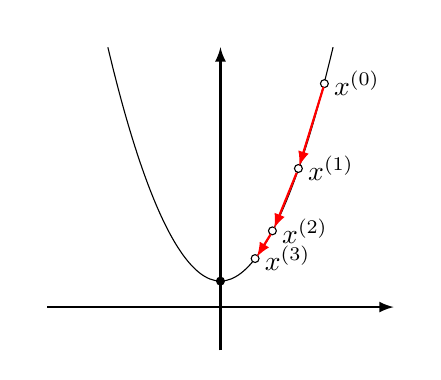
\begin{tikzpicture}[scale=1.1]

    \draw[->=stealth, thick] (0,0)--(2,0) node[right]            {};
    \draw[thick] (0,0)--(-2,0) node[left] {};
    \draw[->=stealth, thick] (0,-0.5)--(0,3) node[above]{};

    \draw (0,0.3) parabola (1.3,3);
    \draw (0,0.3) parabola (-1.3,3);
    \draw[black,fill=black] (0,0.3) circle (.3ex);
    
    \draw[black,fill=white] (1.2,2.58) circle (.3ex) node[right] {\(x^{(0)}\)};
    \draw[black,fill=white] (0.9,1.6) circle (.3ex) node[right] {\(x^{(1)}\)};
    \draw[black,fill=white] (0.6,0.88) circle (.3ex) node[right] {\(x^{(2)}\)};
    \draw[black,fill=white] (0.4,0.56) circle (.3ex) node[right] {\(x^{(3)}\)};
    
    \draw[->=stealth,red,thick] (1.19,2.54)--(0.91,1.63);
    \draw[->=stealth,red,thick] (0.88,1.55)--(0.62,0.91);
    \draw[->=stealth,red,thick] (0.58,0.84)--(0.42,0.58);
    
    \end{tikzpicture}\hspace{0.2in}
    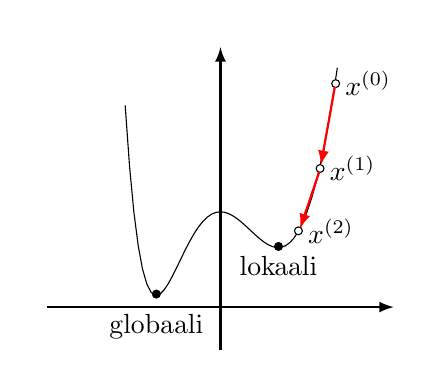
\begin{tikzpicture}[xscale=1,yscale=1,domain=-1.1:1.35,samples=50,scale=1.1]
    \draw[->=stealth, thick] (0,0)--(2,0) node[right]            {};
    \draw[thick] (0,0)--(-2,0) node[left] {};
    \draw[->=stealth, thick] (0,-0.5)--(0,3) node[above]{};
    
    \draw[black] plot (\x,{1.1+2.5*(-\x-1)*(-\x+1)*\x*\x*exp(-0.6*\x)});
    
    \draw[black,fill=white] (1.33,2.58) circle (.3ex) node[right] {\(x^{(0)}\)};
    \draw[black,fill=white] (1.15,1.6) circle (.3ex) node[right] {\(x^{(1)}\)};
    \draw[black,fill=white] (0.9,0.88) circle (.3ex) node[right] {\(x^{(2)}\)};
    
    \draw[->=stealth,red,thick] (1.32,2.54)--(1.16,1.64);
    \draw[->=stealth,red,thick] (1.14,1.56)--(0.92,0.91);
    
        \draw[black,fill=black] (0.67,0.7) circle (.3ex) node[below] {lokaali};

    \draw[black,fill=black] (-0.74,0.15) circle (.3ex) node[below=0.05in] {globaali};
    
    \end{tikzpicture}
\vspace{0.1in}
\\Kuva 7: Gradienttilaskeutuminen konveksille ja ei-konveksille funktiolle
\end{center}

Tarkastellaan sitten gradienttilaskeutumisen soveltamista virhefunktion \(J(W, b)\) minimin määrittämiseksi. Kokonaisvirhefunktio on painoparametrien \(w_{ij}^{(l)}\) ja biasparametrien \(b_i^{(l)}\) funktio, joten skalaarimuodossa voidaan nyt kirjoittaa gradienttilaskeutumisen päivityssäännöt \begin{equation} \label{Wpaiv} w_{ij}^{(l)}\leftarrow w_{ij}^{(l)}-\alpha \frac{\partial J(W, b)}{\partial w_{ij}^{(l)}},\end{equation}
\begin{equation} \label{bpaiv} b_i^{(l)}\leftarrow b_i^{(l)}-\alpha \frac{\partial J(W, b)}{\partial b_i^{(l)}}.\end{equation}
Osittaisderivaatoille voidaan edelleen kirjoittaa \[\begin{align*}
    \frac{\partial J(W, b)}{\partial w_{ij}^{(l)}}&=\frac{\partial}{\partial w_{ij}^{(l)}} \left\{\left[\frac{1}{M}\sum_{i=1}^{M} J(W, b; x^{(i)}, y^{(i)})\right]+\frac{\lambda}{2}\sum_{l=1}^{n_l-1}\sum_{i=1}^{s_l}\sum_{j=1}^{s_{l+1}} \left(w_{ji}^{(l)}\right)^2\right\}\\
    &=\frac{1}{M}\frac{\partial}{\partial w_{ij}^{(l)}} \left[\sum_{i=1}^{M} J(W, b; x^{(i)}, y^{(i)})\right]+\frac{\lambda}{2}\frac{\partial}{\partial w_{ij}^{(l)}} \left[\sum_{l=1}^{n_l-1}\sum_{i=1}^{s_l}\sum_{j=1}^{s_{l+1}} \left(w_{ji}^{(l)}\right)^2\right]\\
    &=\frac{1}{M} \sum_{i=1}^{M} \frac{\partial J(W, b; x^{(i)}, y^{(i)})}{\partial w_{ij}^{(l)}}+\frac{\lambda}{2} \sum_{l=1}^{n_l-1} \sum_{i=1}^{s_l} \sum_{j=1}^{s_l+1} \frac{\partial (w_{ji}^{(l)})^2}{\partial w_{ij}^{(l)}}\\
    &=\frac{1}{M} \sum_{i=1}^{M} \frac{\partial J(W, b; x^{(i)}, y^{(i)})}{\partial w_{ij}^{(l)}}+\lambda \sum_{l=1}^{n_l-1} \sum_{i=1}^{s_l} \sum_{j=1}^{s_l+1} w_{ji}^{(l)}\frac{\partial w_{ji}^{(l)}}{\partial w_{ij}^{(l)}}\\
    &=\frac{1}{M} \sum_{i=1}^{M} \frac{\partial J(W, b; x^{(i)}, y^{(i)})}{\partial w_{ij}^{(l)}}+\lambda w_{ij}^{(l)},
\end{align*}\]
\[\begin{align*}
    \frac{\partial J(W, b)}{\partial b_{i}^{(l)}}&=\frac{\partial}{\partial b_{i}^{(l)}} \left\{\left[\frac{1}{M}\sum_{i=1}^{M} J(W, b; x^{(i)}, y^{(i)})\right]+\frac{\lambda}{2}\sum_{l=1}^{n_l-1}\sum_{i=1}^{s_l}\sum_{j=1}^{s_{l+1}} \left(w_{ji}^{(l)}\right)^2\right\}\\
    &=\frac{1}{M}\frac{\partial}{\partial b_{i}^{(l)}} \left[\sum_{i=1}^{M} J(W, b; x^{(i)}, y^{(i)})\right]+\frac{\lambda}{2}\frac{\partial}{\partial b_{i}^{(l)}} \left[\sum_{l=1}^{n_l-1}\sum_{i=1}^{s_l}\sum_{j=1}^{s_{l+1}} \left(w_{ji}^{(l)}\right)^2\right]\\
    &=\frac{1}{M} \sum_{i=1}^{M} \frac{\partial J(W, b; x^{(i)}, y^{(i)})}{\partial b_{i}^{(l)}}+\frac{\lambda}{2} \sum_{l=1}^{n_l-1} \sum_{i=1}^{s_l} \sum_{j=1}^{s_l+1} \frac{\partial (w_{ji}^{(l)})^2}{\partial b_{i}^{(l)}}\\
    &=\frac{1}{M} \sum_{i=1}^{M} \frac{\partial J(W, b; x^{(i)}, y^{(i)})}{\partial b_{i}^{(l)}}.
\end{align*}\]
Tarvitaan siis \(\displaystyle \frac{\partial J(W, b; x^{(i)}, y^{(i)})}{\partial w_{ij}^{(l)}}\) ja \(\displaystyle \frac{\partial J(W, b; x^{(i)}, y^{(i)})}{\partial b_{i}^{(l)}}\) eli virhefunktion osittaisderivaatat kunkin painon ja biaksen suhteen, jotka voidaan määrittää vastavirta-algoritmin (\textit{backpropagation}) avulla.

\subsection{Vastavirta-algoritmi}
Tarkastellaan osittaisderivaattojen määräämistä selkeyden vuoksi ensin esimerkin avulla kuvan 6 neuroverkolle. Aloitetaan tarkastelu lähtökerroksesta ja edetään tästä muihin kerroksiin. Lopuksi päättely yleistetään ja muotoillaan matriisiesityksenä.

\subsubsection{Lähtökerros}
Aloitetaan lähtökerroksesta ja määrätään virhefunktion osittaisderivaatta parametrin \(w_{12}^{(2)}\) suhteen, joka on siis piilokerroksen neuronin 2 ja lähtökerroksen ainoan neuronin 1 välisen linkin paino. Tarkastelemalla virhefunktion lauseketta havaitaan kuitenkin, että ei ole suoraan selvää, miten \(J\) riippuu parametrista \(w_{12}^{(2)}\). Soveltamalla ketjusääntöä voidaan kuitenkin kirjoittaa \begin{equation} \label{virhe} \frac{\partial J}{\partial w_{12}^{(2)}}=\frac{\partial J}{\partial h_1^{(3)}} \frac{\partial h_1^{(3)}}{\partial w_{12}^{(2)}}=\frac{\partial J}{\partial h_1^{(3)}} \frac{\partial h_1^{(3)}}{\partial z_1^{(3)}} \frac{\partial z_1^{(3)}}{\partial w_{12}^{(2)}},\end{equation} jossa \[\frac{\partial z_1^{(3)}}{\partial w_{12}^{(2)}}=\frac{\partial}{\partial w_{12}^{(2)}}(w_{11}^{(2)} h_1^{(2)}+w_{12}^{(2)} h_2^{(2)}+w_{13}^{(2)} h_3^{(2)}+b_1^{(2)})=h_2^{(2)}\frac{\partial w_{12}^{(2)}}{\partial w_{12}^{(2)}}=h_2^{(2)}\] ja edelleen \[\frac{\partial h_1^{(3)}}{\partial z_1^{(3)}}=\frac{\partial f(z_1^{(3)})}{\partial z_1^{(3)}}=\frac{\partial z_1^{(3)}}{\partial z_1^{(3)}} f'(z_1^{(3)})=f'(z_1^{(3)}).\]
Osittaisderivaataksi verkon lähdön suhteen saadaan lopulta \[\frac{\partial J}{\partial h_1^{(3)}}=\frac{\partial}{\partial h_1^{(3)}} \left(\frac{1}{2}\norm{y_1-h_1^{(3)}}^2\right)=\frac{\partial (y_1-h_1^{(3)})}{\partial h_1^{(3)}}\cdot (y_1-h_1^{(3)})=-(y_1-h_1^{(3)}).\] Määritellään nyt \[\delta_1^{(3)}=\frac{\partial J}{\partial h_1^{(3)}}\frac{\partial h_1^{(3)}}{\partial z_1^{(2)}}=-(y_1-h_1^{(3)})\cdot f'(z_1^{(3)}),\] jolloin alkuperäinen osittaisderivaatta \ref{virhe} voidaan kirjoittaa muodossa \[\frac{\partial J}{\partial w_{12}^{(2)}}=h_2^{(2)} \delta_1^{(3)}.\]
\begin{huom}
Voidaan tulkita, että \(\delta_1^{(3)}\) kuvaa sitä osuutta, joka kerroksen 3 (lähtökerros) neuronilla 1 on verkon tekemään virheeseen.
\end{huom}

Vastaava päättely voidaan toistaa myös muille lähtökerroksen \(n_l\) ja sen viereisen piilokerroksen \(n_l-1\) välisille painoille, jolloin voidaan kirjoittaa yleisemmin \[\frac{\partial J}{\partial w_{ij}^{(n_l-1)}}=h_j^{(n_l-1)}\delta_i^{(n_l)},\text{ jossa } \delta_i^{(n_l)}=-(y_i-h_i^{(n_l)})\cdot f'(z_i^{(n_l)}).\]

Tarkastellaan sitten hieman vastaavasti osittaisderivaattaa lähtökerroksen neuronin 1 biaksen \(b_1^{(2)}\) suhteen. Nyt jälleen ketjusäännön nojalla

\[\frac{\partial J}{\partial b_{1}^{(2)}}=\underbrace{\frac{\partial J}{\partial z_1^{(2)}}}_{=\delta_1^{(3)}} \frac{\partial z_1^{(2)}}{\partial b_1^{(2)}},\] jossa \[\frac{\partial z_1^{(2)}}{\partial b_1^{(2)}}=\frac{\partial}{\partial b_1^{(2)}} (w_{11}^{(2)}h_1^{(2)}+w_{12}^{(2)}h_2^{(2)}+w_{13}^{(2)}h_3^{(2)}+b_1^{(2)})=\frac{\partial b_1^{(2)}}{\partial b_1^{(2)}}=1\] ja näin ollen \[\frac{\partial J}{\partial b_1^{(2)}}=\delta_1^{(3)}\cdot 1=\delta_1^{(3)}.\] Vastaava päättely voidaan toistaa kaikille lähtökerroksen neuroneille, jolloin saadaan \[\frac{\partial J}{\partial b_{i}^{(n_l-1)}}=\delta_i^{(n_l)}.\]

\subsubsection{Piilokerrokset}
Edellä osittaisderivaattojen määrittäminen painojen ja biasten suhteen onnistui suoraviivaisesti, sillä lähtökerroksen neuronit tuottavat koko verkon lähdön ja siten niiden lähtöjä voidaan verrata suoraan todelliseen arvoon. Piilokerrosten osalta tilanne poikkeaa tästä, sillä ne eivät tuota suoraan verkon lähtöä, vaan piilokerrosten neuronien lähdöt vaikuttavat verkon lähtöön muiden neuronien välityksellä. Esimerkiksi kerroksen 2 neuroni 1 vaikuttaa lähtökerroksen neuroneihin ja tätä kautta koko verkon lähtöön. Tätä on havainnollistettu kuvassa 8.

\begin{center}
\tikzset{%
  every neuron/.style={
    circle,
    draw,
    minimum size=1cm
  },
  neuron missing/.style={
    draw=none, 
    scale=3,
    text height=0.333cm,
    execute at begin node=\color{black}$\vdots$
  },
}

\begin{tikzpicture}[x=1.5cm, y=1.5cm, >=stealth]


\foreach \m/\l [count=\y] in {1,2,3,4}
  \node [every neuron/.try, neuron \m/.try] (input-\m) at (0,2.5-\y) {};

\node [every neuron/.try, neuron \m/.try,red] (hidden-\m) at (2,2.5-1*1.25) {};
\foreach \m [count=\y] in {2,3}
  \node [every neuron/.try, neuron \m/.try] (hidden-\m) at (2,2.5-\y*1.25-1.25) {};

\foreach \m [count=\y] in {1,2}
  \node [every neuron/.try, neuron \m/.try,blue] (output-\m) at (4,1.5-\y) {};

\foreach \l [count=\i] in {1,2,3,4}
  \draw [<-] (input-\i) -- ++(-1.5,0)
    node [left,inner sep=0.2cm] {$x_\l$};
  %\node[] at (0,1.5) {\(x_2\)};
  
\foreach \l [count=\i] in {1,2,3,4}
  \filldraw (input-\i)++(-1.5,0) circle (2pt);
    
\foreach \l [count=\i] in {1,2,3,4} % syötekerroksen numerot
  \node [shift={(0,-0.34)}] at (input-\i.north) {\l};

\foreach \l [count=\i] in {1,2,3} % piilokerroksen numerot
  \node [shift={(0,-0.34)}] at (hidden-\i.north) {\l};
  
\foreach \l [count=\i] in {1,2} % lähtökerroksen numerot
  \node [shift={(0,-0.34)}] at (output-\i.north) {\l};

\foreach \l [count=\i] in {1,2}
  \draw [->] (output-\i) -- ++(1.5,0)
    node [right,inner sep=0.2cm] {$h_\l^{(3)}$};


\foreach \l [count=\i] in {1,2}
    \filldraw (output-\i)++(1.5,0) circle (2pt);

\foreach \i in {1,...,4}
  \foreach \j in {1,...,3}
    \draw [->] (input-\i) -- (hidden-\j);

\draw [->,red] (hidden-1) -- (output-1);
\draw [->,red] (hidden-1) -- (output-2);
\foreach \i in {2,...,3}
  \foreach \j in {1,...,2}
    \draw [->] (hidden-\i) -- (output-\j);

\foreach \l [count=\x from 0] in {syötekerros\\ \(L_1\), piilokerros\\ \(L_2\), lähtökerros\\ \(L_3\)}
  \node [align=center, above] at (\x*2,2) {\l};

\end{tikzpicture}
\vspace{0.1in}
\\Kuva 8: Piilokerroksen neuronin välillinen vaikutus verkon lähtöön
\end{center}

Tarkastellaan nyt esimerkkinä osittaisderivaattaa painon \(w_{11}^{(1)}\) eli syöte- ja piilokerrosten neuronien 1 linkin välisen painon suhteen. Sovelletaan jälleen ketjusääntöä, mutta nyt on huomioitava kaikki neuronit, jotka riippuvat kerroksen 2 neuronista 1 eli käyttävät tämän neuronin lähtöä syötteenään. Kirjoitetaan nyt ensin ketjusäännön nojalla \[\frac{\partial J}{\partial w_{11}^{(1)}}=\frac{\partial J}{\partial z_1^{(2)}} \frac{\partial z_1^{(2)}}{\partial w_{11}^{(1)}}.\]
Tutkitaan saadun tulon ensimmäistä osittaisderivaattaa. Koska kerroksen 2 neuronista 1 riippuvat nyt suoraan kerroksen 3 neuronit 1 ja 2, joiden summainten lähdöt ovat \(z_1^{(3)}\) ja \(z_2^{(3)}\), kirjoitetaan ketjusäännön nojalla \begin{equation}\label{Jz} \frac{\partial J}{\partial z_1^{(2)}}=\sum_{i=1}^{2} \underbrace{\frac{\partial J}{\partial z_i^{(3)}}}_{=\delta_i^{(3)}} \frac{\partial z_i^{(3)}}{\partial z_1^{(2)}}=\sum_{i=1}^{2} \delta_i^{(3)} \frac{\partial z_i^{(3)}}{\partial h_1^{(2)}} \frac{\partial h_1^{(2)}}{\partial z_1^{(2)}}.\end{equation} Osittaisderivaatoille havaitaan suoralla laskulla, että \[\frac{\partial z_i^{(3)}}{\partial h_1^{(2)}}=\frac{\partial}{\partial h_1^{(2)}}(w_{i1}^{(2)} h_1^{(2)} + w_{i2}^{(2)} h_2^{(2)} + w_{i3}^{(2)} h_3^{(2)} + b_i^{(2)})=w_{i1}^{(2)}\] ja \[\frac{\partial h_1^{(2)}}{\partial z_1^{(2)}}=\frac{\partial f(z_1^{(2)})}{\partial z_1^{(2)}}=\frac{\partial z_1^{(2)}}{\partial z_1^{(2)}} f'(z_1^{(2)})=f'(z_1^{(2)}).\] Sijoittamalla nämä lausekkeeseen \ref{Jz} voidaan todeta, että \[\frac{\partial J}{\partial z_1^{(2)}}=\sum_{i=1}^{2} \delta_i^{(3)}w_{i1}^{(2)}\cdot f'(z_1^{(2)})=\left(\sum_{i=1}^{2} w_{i1}^{(2)} \delta_i^{(3)}\right) f'(z_1^{(2)})=\delta_1^{(2)}.\] Tämä on virhetermi kerroksen 2 neuronille 1. Edelleen suoralla laskulla \[\frac{\partial z_1^{(2)}}{\partial w_{11}^{(1)}}=\frac{\partial}{\partial w_{11}^{(1)}}(w_{11}^{(1)} h_1^{(1)}+w_{12}h_2^{(1)}+w_{13}^{(1)}h_3^{(1)})=h_1^{(1)},\] joten lopulta \[\frac{\partial J}{\partial w_{11}^{(1)}}=h_1^{(1)} \delta_1^{(2)}.\] Todetaan siis, että osittaisderivaatalle piilokerroksen painon suhteen saatiin vastaava lauseke kuin edellisessä kohdassa lähtökerroksen painolle: erona on ainoastaan virhetermin \(\delta\) laskentatapa. Erityisesti havaitaan, että virhetermit riippuvat nyt edellä tarkastellun lähtökerroksen neuronien virhetermeistä.

Osoittautuukin, että tämänkaltainen rekursiivinen päättely voidaan yleistää. Kerroksen \(l\) neuronien virhetermit saadaan nimittäin kerroksen \(l+1\) neuronien virhetermeistä lausekkeella \[\delta_j^{(l)}=\left(\sum_{i=1}^{s_{l+1}} w_{ij}^{(l)} \delta_i^{(l+1)}\right) f'(z_j^{(l)}).\] Vastaavasti osittaisderivaatat yleisen painon ja biaksen suhteen ovat tällöin \[\frac{\partial J}{\partial w_{ij}^{(l)}}=h_j^{(l)} \delta_i^{(l+1)}, \ \ \frac{\partial J}{\partial b_i^{(l)}}=\delta_i^{(l+1)}.\]
Vastavirta-algoritmi etenee siis siten, että ensin määrätään lähtökerroksen neuroneille virhetermit \(\delta_i^{(n_l)}\), joiden avulla saadaan lähtökerrosta lähinnä olevan piilokerroksen virhetermit \(\delta_i^{(n_l-1)}\). Näin jatkamalla saadaan rekursiivisesti määrättyä kaikki virhetermit ja niiden avulla suoraviivaisesti halutut osittaisderivaatat kaikkien painojen ja biasten suhteen.

\subsubsection{Matriisimuoto}
Selkeyden ja laskentatehokkuuden vuoksi vastavirta-algoritmin lausekkeet on hyödyllistä kirjoittaa matriisimuodossa myötäsyöttöalgoritmin tapaan. Määrittelemällä virhetermivektori \[\delta^{(i)}=\begin{bmatrix} \delta_1^{(i)} & \delta_2^{(i)} & \cdots & \delta_{s_i}^{(i)}\end{bmatrix}^{\top}\] voidaan lähtökerrokselle kirjoittaa suorana yleistyksenä \[\delta^{(n_l)}=-(y-h^{(n_l)})\odot f'(z^{(n_l)}).\] Tässä merkinnällä \(A\odot B\) tarkoitetaan matriisitulon sijaan Hadamard-tuloa eli alkiokohtaista tuloa, jossa tulosmatriisin rivin \(i\) sarakkeen \(j\) alkio saadaan kertomalla keskenään alkiot \(A_{ij}\) ja \(B_{ij}\).

Edelleen, kun määritellään lisäksi painomatriisi \(W^{(l)}\) ja lähtövektori \(z^{(l)}\) kuten myötäsyöttöprosessissa, voidaan muille kerroksille kirjoittaa \[\delta^{(l)}=\left[(W^{(l)})^{\top} \delta^{(l+1)}\right]\odot f'(z^{(l)}).\]
Todetaan, että nyt esimerkiksi \[\begin{align*}
\delta^{(2)}&=\left[(W^{(2)})^{\top} \delta^{(3)}\right]\odot f'(z^{(2)})\\
&=\left( \begin{bmatrix} w_{11}^{(2)} & w_{12}^{(2)} & w_{13}^{(2)} \\ w_{21}^{(2)} & w_{22}^{(2)} & w_{23}^{(2)} \end{bmatrix}^{\top} \begin{bmatrix} \delta_1^{(3)} \\ \delta_2^{(3)}\end{bmatrix}\right) \odot \begin{bmatrix} f'(z_1^{(2)}) \\ f'(z_2^{(2)}) \\ f'(z_3^{(2)}) \end{bmatrix}\\
&=\left( \begin{bmatrix} w_{11}^{(2)} & w_{21}^{(2)} \\
w_{12}^{(2)} & w_{22}^{(2)} \\ w_{13}^{(2)} & w_{23}^{(2)}
\end{bmatrix} \begin{bmatrix} \delta_1^{(3)} \\ \delta_2^{(3)}\end{bmatrix}\right) \odot \begin{bmatrix} f'(z_1^{(2)}) \\ f'(z_2^{(2)}) \\ f'(z_3^{(3)}) \end{bmatrix}\\
&=\begin{bmatrix}\displaystyle
\sum_{i=1}^{2} w_{i1}^{(2)} \delta_i^{(3)}\\
\displaystyle \sum_{i=1}^{2} w_{i2}^{(2)} \delta_i^{(3)}\\
\displaystyle \sum_{i=1}^{2} w_{i3}^{(2)} \delta_i^{(3)}
\end{bmatrix}\odot \begin{bmatrix} f'(z_1^{(2)}) \\ f'(z_2^{(2)}) \\ f'(z_3^{(3)}) \end{bmatrix}
=\begin{bmatrix}\displaystyle
\left(\sum_{i=1}^{2} w_{i1}^{(2)} \delta_i^{(3)}\right) f'(z_1^{(2)})\\
\displaystyle \left(\sum_{i=1}^{2} w_{i2}^{(2)} \delta_i^{(3)}\right) f'(z_2^{(2)})\\
\displaystyle \left(\sum_{i=1}^{2} w_{i3}^{(2)} \delta_i^{(3)}\right) f'(z_3^{(2)})
\end{bmatrix}.
\end{align*}\]
Osittaisderivaatoille voidaan tällöin kirjoittaa \begin{equation} \label{Wosit} \frac{\partial J}{\partial W^{(l)}}=\delta_i^{(l+1)} (h^{(l)})^{\top},\end{equation}
\begin{equation}\label{bosit} \frac{\partial J}{\partial b^{(l)}}=\delta^{(l+1)}.\end{equation}
Prosessi voidaan muotoilla oheiseksi algoritmiksi.
\begin{algorithm}[H]
\renewcommand{\thealgorithm}{2}
    \caption{(Vastavirta-algoritmi)}
    \begin{algorithmic}[1]
        \Input \State \multiline{%
        opetusesimerkki $(x, y)$, painomatriisit $W^{(i)}$ ja biasvektorit $b^{(i)}$,\\$i=1,2,\ldots, n_l$}
        \Step \State Suoritetaan myötäsyöttö syötteellä $x$ (ks. Algoritmi 1)
        \Step \State $\delta^{(n_l)}=-(y-h^{(n_l)})\odot f'(z^{(n_l)})$
        \Step \State \textbf{jokaiselle} {$l=n_l-1, n_l-2,\ldots,2$:}
        \NoNumber \State \qquad {$\delta^{(l)}=\left[(W^{(l)})^{\top} \delta^{(l+1)}\right]\odot f'(z^{(l)})$}
        \EndFor
        \Step \State $\partial J / \partial W^{(l)}=\delta^{(l+1)} (h^{(l)})^{\top}$ kaikille $l$
        \Step \State $\partial J / \partial b^{(l)}=\delta^{(l+1)}$
        \Output \State \multiline{%
        osittaisderivaatat $\partial J / \partial W^{(l)}=\delta_i^{(l+1)} (h^{(l)})^{\top}$ ja $\partial J / \partial b^{(l)}=\delta^{(l+1)}$\\kaikille $l$}
    \end{algorithmic}
\end{algorithm}

\subsection{Opetusalgoritmi}
Edellä määrättiin yksittäiselle esimerkille kirjoitetulle virhefunktiolle \(J(W, b; x^{(i)}, y^{(i)})\) osittaisderivaatat painojen ja biasten suhteen vektorimuodossa. Palataan nyt tarkastelemaan kokonaisvirhefunktiota \(J(W, b)\) ja kirjoitetaan gradienttilaskeutumisen päivityssäännöt \ref{Wpaiv}, \ref{bpaiv} vektorimuodossa:
\begin{equation} \label{Wkok} W^{(l)}\leftarrow W^{(l)} - \alpha\left[\frac{1}{M} \underbrace{\sum_{i=1}^{M} \frac{\partial J(W, b; x^{(i)}, y^{(i)})}{\partial W^{(l)}}}_{\Delta W^{(l)}}+\lambda W^{(l)}\right],\end{equation}
\begin{equation} \label{bkok} b^{(l)}\leftarrow b^{(l)} - \alpha\left[\frac{1}{M} \underbrace{\sum_{i=1}^{M} \frac{\partial J(W, b; x^{(i)}, y^{(i)})}{\partial b^{(l)}}}_{\Delta b^{(l)}}\right].\end{equation}
Päivityssääntöjä varten tarvitaan siis summat jokaisen opetusesimerkin \(i\) suhteen virhefunktion \(J(W, b; x^{(i)}, y^{(i)})\) osittaisderivaatoista, ts. \(\Delta W^{(l)}\) ja \(\Delta b^{(l)}\).

Opetusalgoritmissa nämä summat lasketaan vaiheittain. Aluksi painomatriisit ja biasvektorit alustetaan satunnaisiin, pieniin arvoihin, jotka voidaan valita esimerkiksi normaalijakaumalta; vastaavasti summatermit \(\Delta W^{(l)}\) ja \(\Delta b^{(l)}\) alustetaan nolliksi. Tämän jälkeen käydään läpi kaikki opetusesimerkit. Kunkin opetusesimerkin \(i\) syötteelle \(x^{(i)}\) suoritetaan myötäsyöttöprosessi ja kerrosten \(h^{(l)}\) lähdöt otetaan talteen. Näiden ja vastavirta-algoritmin avulla voidaan edelleen laskea virhetermivektorit \(\delta^{(l)}\) kaikille kerroksille. Lopulta summia \(\Delta W^{(l)}\) ja \(\Delta b^{(l)}\) kerrytetään kullekin kerrokselle lisäämällä niihin virhefunktion osittaisderivaatat, jotka saadaan yhtälöistä \ref{Wosit}, \ref{bosit}: \[\Delta W^{(l)}\leftarrow \Delta W^{(l)}+\frac{\partial J(W, b; x^{(i)}, y^{(i)})}{\partial W^{(l)}}=\Delta W^{(l)}+\delta^{(l+1)}(h^{(l)})^{\top},\]
\[\Delta b^{(l)}\leftarrow \Delta b^{(l)}+\frac{\partial J(W, b; x^{(i)}, y^{(i)})}{\partial b^{(l)}}=\Delta b^{(l)}+\delta^{(l+1)}.\]

Kun kaikki opetusesimerkit on käyty läpi, voidaan painot ja biakset päivittää lopulta säännöillä \ref{Wkok}, \ref{bkok}: \[W^{(l)}\leftarrow W^{(l)} - \alpha\left[\frac{1}{M} \Delta W^{(l)}+\lambda W^{(l)}\right],\]
\[b^{(l)}\leftarrow b^{(l)} - \alpha\left[\frac{1}{M} \Delta b^{(l)}\right].\]
Tämä muodostaa algoritmin yhden iteraation. Iterointia voidaan jatkaa esimerkiksi ennalta määritellyn iteraatiolukumäärän verran tai kunnes opetusdatalle tehty ennustevirhe on riittävän pieni. Koko opetusalgoritmi on kuvattu alla.
\begin{algorithm}[H]
\renewcommand{\thealgorithm}{3}
    \caption{(Opetusalgoritmi)}
    \begin{algorithmic}[1]
        \Input \State
        \multiline{%
        opetusdatajoukko $L=\{(x^{(1)}, y^{(1)}), (x^{(2)}, y^{(2)}), \ldots, (x^{(M)}, y^{(M)})\}$,\\ painotuskerroin $\lambda$, oppimisnopeus $\alpha$}
        \vspace{0.1in}
        \Step \State \multiline{%
        Alustetaan kaikki painomatriisit $W^{(l)}$ ja biasvektorit $b^{(l)}$\\satunnaisluvuilla}
        \Step \State Alustetaan $\Delta W^{(l)}$ ja $\Delta b^{(l)}$ nolliksi kaikille $l$\\
        \Step \textbf{jokaiselle} {$(x^{(i)}, y^{(i)})\in L$:}
        \NoNumber \State \qquad {a. Suoritetaan myötäsyöttö syötteellä $x^{(i)}$ (ks. Algoritmi 1)}
        \NoNumber \State \qquad \multiline{%
        {b. Lasketaan vastavirta-algoritmilla virhevektorit $\delta^{(l)}$\\ \quad (ks. Algoritmi 2)}}
        \NoNumber \State \qquad c. $\Delta W^{(l)}\leftarrow \Delta W^{(l)}+\delta^{(l+1)}(h^{(l)})^{\top}$ kaikille $l$
        \NoNumber \State \qquad d. $\Delta b^{(l)}\leftarrow \Delta b^{(l)}+\delta^{(l+1)}$ kaikille $l$
        \EndFor
        \Step \State $\displaystyle W^{(l)}\leftarrow W^{(l)} - \alpha\left[\frac{1}{M} \Delta W^{(l)}+\lambda W^{(l)}\right]$
        \Step \State $\displaystyle b^{(l)}\leftarrow b^{(l)} - \alpha\left[\frac{1}{M} \Delta b^{(l)}\right]$
        \Step \State Palataan askeleeseen 2, jos lopetusehtoa ei ole saavutettu
        \vspace{0.1in}
        \Output \State optimaaliset painomatriisit \(W^{(l)}\) ja biasvektorit \(b^{(l)}\)
    \end{algorithmic}
\end{algorithm}

%\renewcommand{\bibname}{Lähdeluettelo}  % Muutetaan lähdeluettelon nimeä; kirjat, raportit
\renewcommand{\refname}{Lähdeluettelo}  % Muutetaan lähdeluettelon nimeä; artikkelit

%\addcontentsline{toc}{section}{\bibname} % Lisätäänn lähdeluettelo sisällysluetteloon; kirjat, raportit
\addcontentsline{toc}{section}{\refname} % Lisätään lähdeluettelo sisällysluetteloon; artikkelit yms.

\begin{thebibliography}{99}
\bibitem{deriv} P. Liskowski: \emph{Derivation of Backpropagation Algorithm
for Feedforward Neural Networks}. URL: \href{http://www.cs.put.poznan.pl/pliskowski/pub/teaching/eio/lab1/eio-supplementary.pdf}{http://www.cs.put.poznan.pl/pliskowski/pub/teaching/eio/lab1/eio-supplementary.pdf}.

\bibitem{net} R. Rojas: \emph{Neural Networks -- A Systematic Introduction}. Springer, 1996.

\bibitem{Z2b} A. Thomas: \emph{An introduction to neural
networks for beginners}. URL: \href{https://adventuresinmachinelearning.com/wp-content/uploads/2017/07/An-introduction-to-neural-networks-for-beginners.pdf}{https://adventuresinmachinelearning.com/wp-content/uploads/2017/07/An-introduction-to-neural-networks-for-beginners.pdf}.

\bibitem{stanf} \emph{Unsupervised Feature Learning and Deep Learning Tutorial: Multi-Layer Neural Networks}. Stanford University. URL: \href{http://ufldl.stanford.edu/tutorial/supervised/MultiLayerNeuralNetworks/}{http://ufldl.stanford.edu/tutorial/supervised/MultiLayerNeuralNetworks/}.
\end{thebibliography}

\end{document}
